\documentclass[12pt]{article}
\usepackage{pdfpages}
\usepackage{setspace}
\usepackage[dutch]{babel}

% Importeer configuratie-instellingen
\RequirePackage{C:/Users/danny/Documents/GitHub/Statistiek/LaTeX/styles/exam_config}
\RequirePackage{C:/Users/danny/Documents/GitHub/Statistiek/LaTeX/styles/statistics-macros}
\graphicspath{{C:/Users/danny/Documents/GitHub/Statistiek/LaTeX/figures/}}

\renewcommand{\baselinestretch}{1.5}
% Begin van het document
\begin{document}

% FMW-specifiek titelblad voordat het examen begint
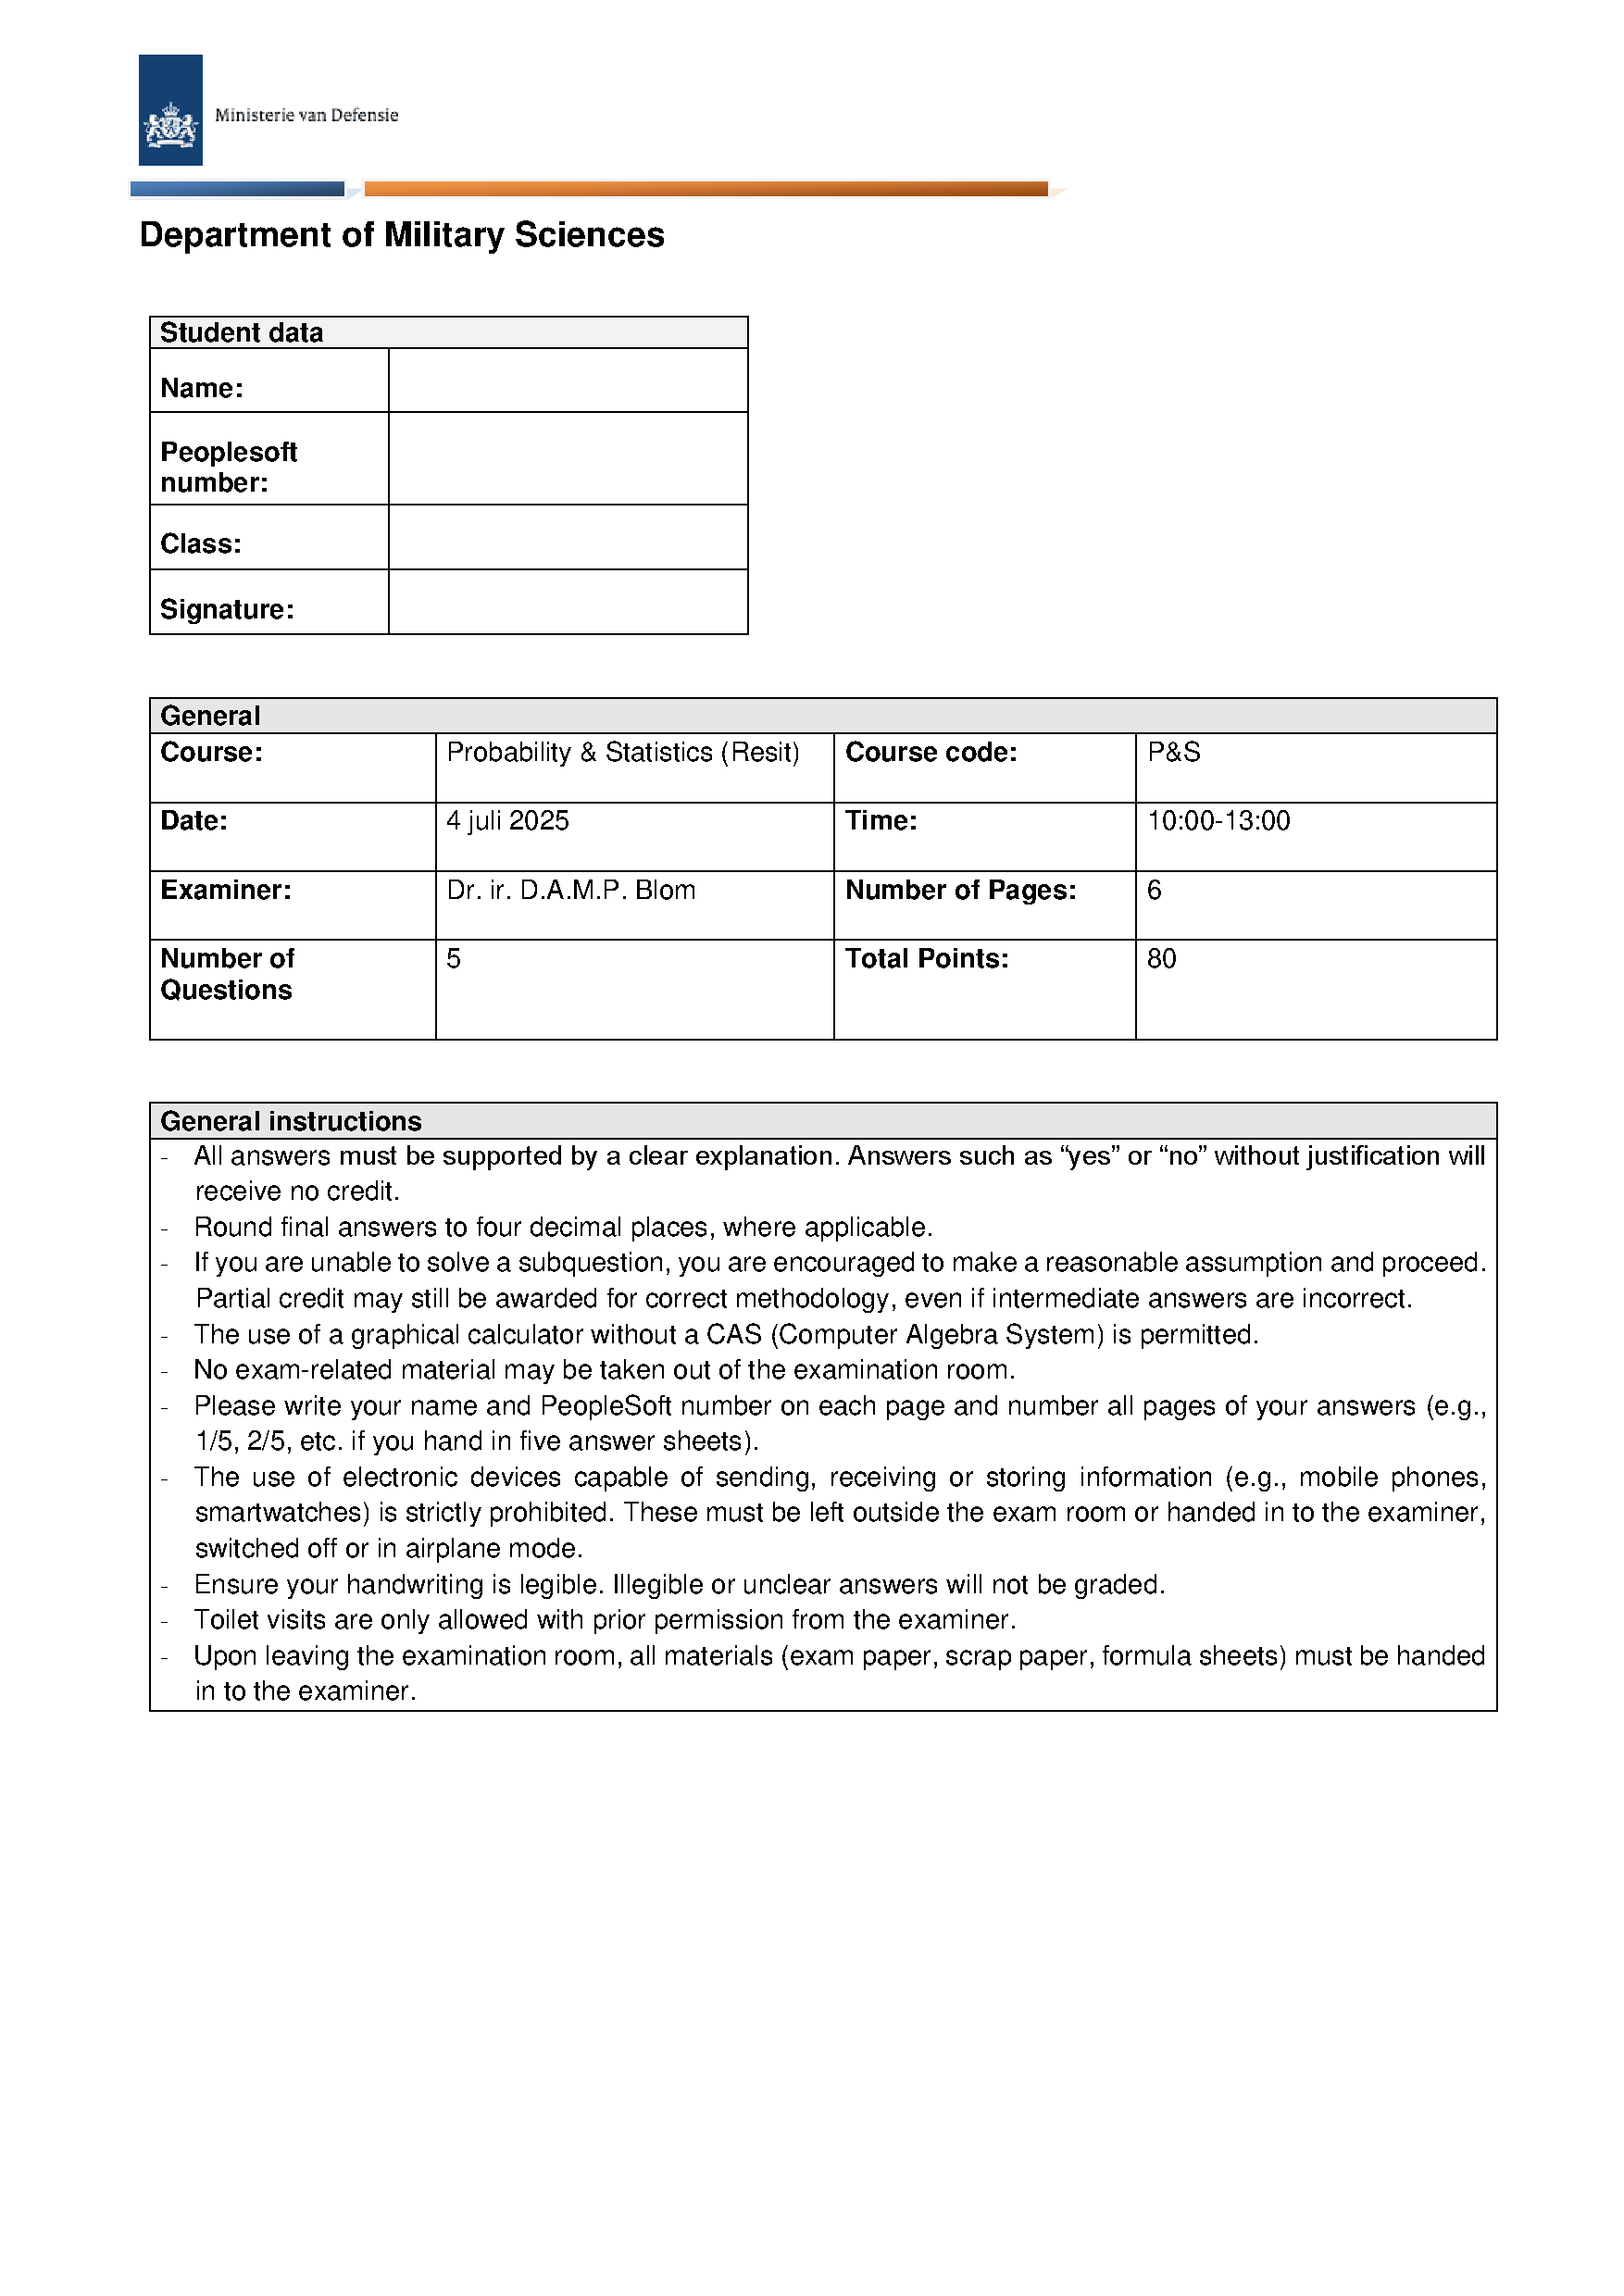
\includepdf[pages=-]{\folder/Python/FMW_titelblad_20250704.pdf}

% \title{Tentamen statistiek}
% \author{Nederlandse Defensie Academie}
% \date{\today}
% \maketitle

% 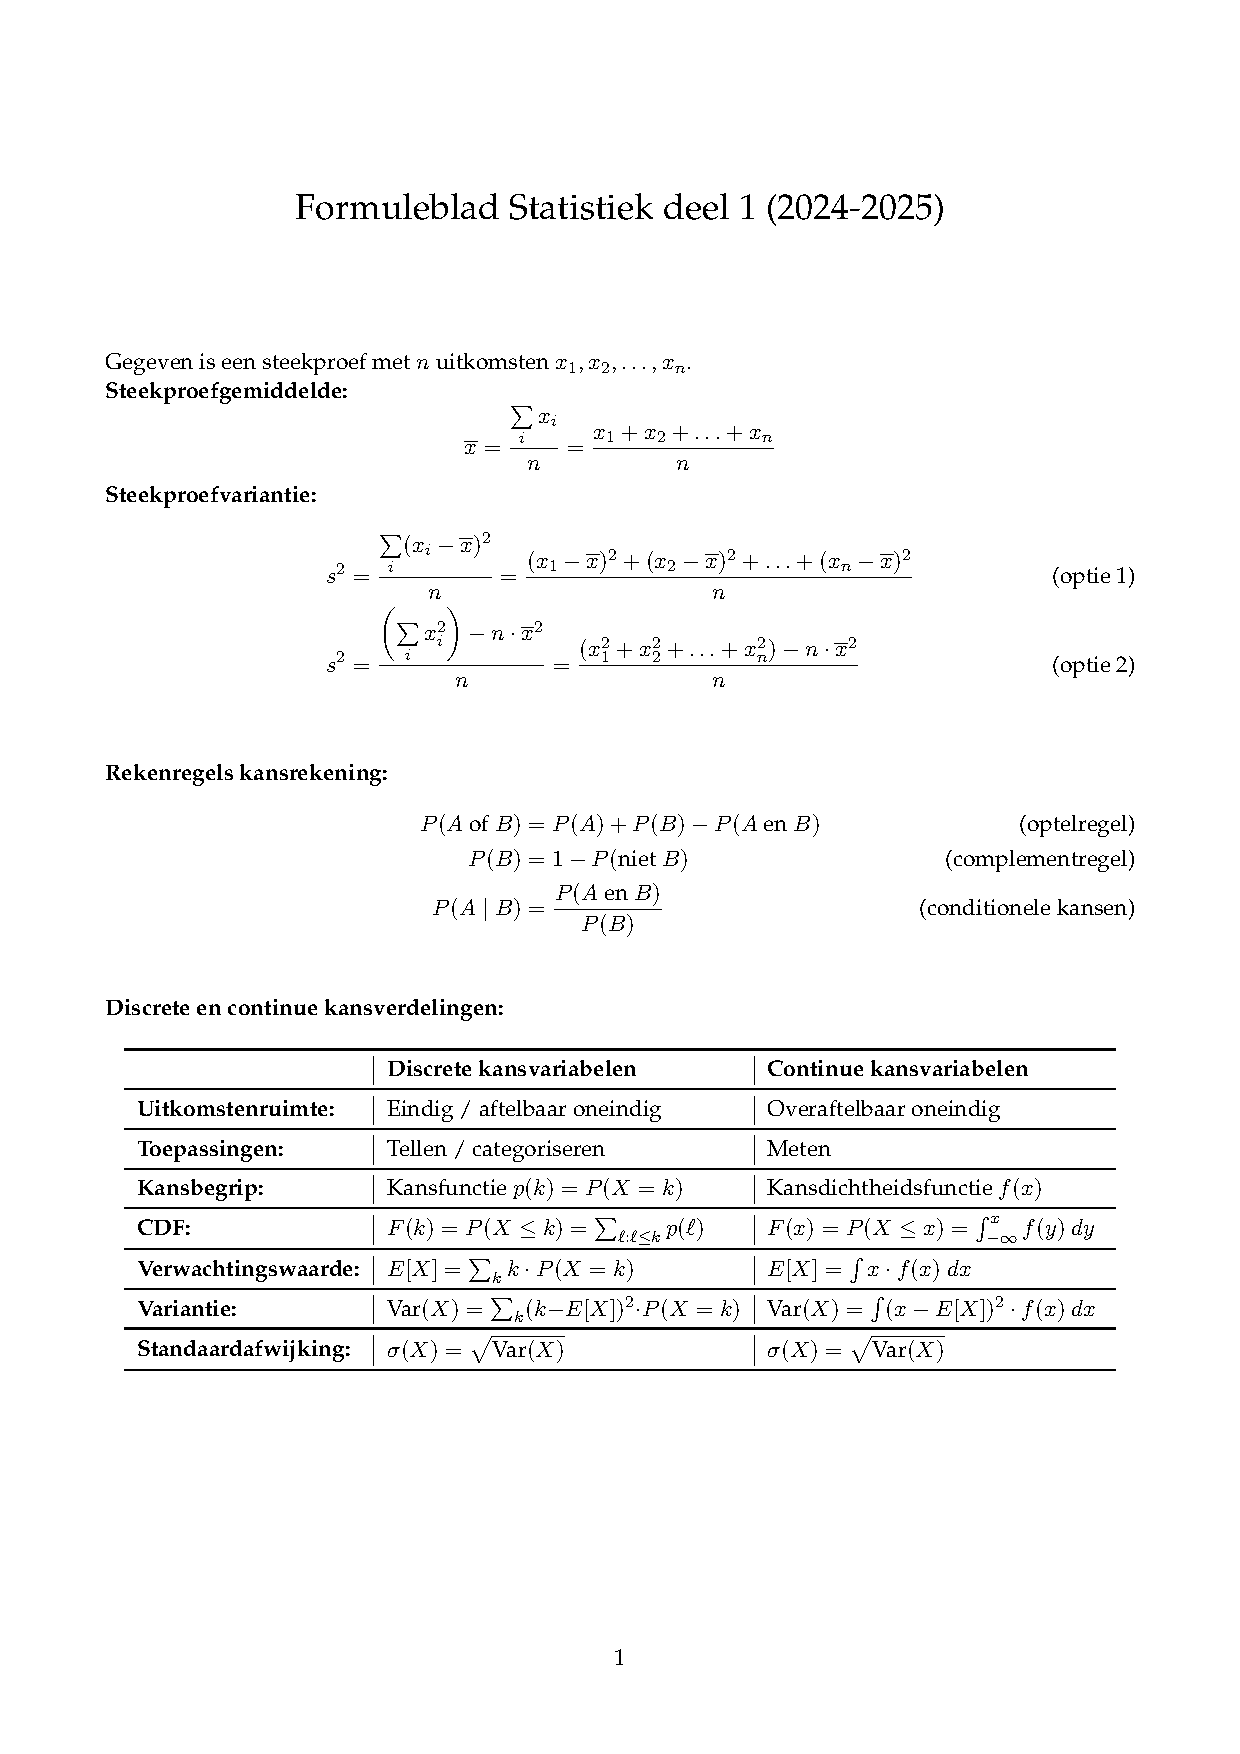
\includepdf[pages=-]{\folder/LaTeX/formulebladen/formuleblad_1.pdf}

% Include questions from external files
\begin{question}{22}{
    Een onderzoeksteam van het Maritime Warfare Center (MWC) onderzoekt de signaalsterkte (in decibel) van sonarpulsen die worden gereflecteerd door een nieuw type onderzeeboot.
    Het huidige ontwerp heeft een gemiddelde gereflecteerde signaalsterkte van $\mu = 65$ decibel.

    Het MWC wil toetsen of het nieuw ontwerp de detecteerbaarheid reduceert, oftewel dat de gereflecteerde signaalsterkte significant lager ligt bij het nieuwe ontwerp.
    In een steekproef van tien onafhankelijke metingen is bij het nieuwe ontwerp de gereflecteerde signaalsterkte in decibel gemeten met gemiddelde $63,75$ decibel en standaardafwijking $s = 0,78$.
    Je mag aannemen dat de signaalsterktes normaal verdeeld zijn met onbekende standaardafwijking $\sigma$.
    
    Gebruik voor de hypothesetoets een significantieniveau van $\alpha=0,05$.
}
    \subquestion{4}{
       Definieer de nulhypothese en de alternatieve hypothese van de hypothesetoets.
       Verklaar het gekozen type (tweezijdig, linkszijdig of rechtszijdig) van de toets.
    }
    \solution{
        Aangezien we willen toetsen of de gemiddelde gereflecteerde signaalsterkte significant lager ligt dan $\mu = 65$, kunnen we de hypothesetoets als volgt defini\"eren:
        \begin{align*}
            H_0&: \mu \ge 65 \quad \text{(geen significante vermindering)} \rubric{2} \\
            H_1&: \mu < 65 \quad \text{(wel een significante vermindering)} \rubric{1}
        \end{align*}
        Dit is een linkszijdige toets, omdat de nulhypothese uitgaat van een status-quo (geen verbetering) en de alternatieve hypothese juist wel een verbetering aanduidt.
         \rubric{1}
    }
    
    \subquestion{4}{
       Voer de bijbehorende hypothesetoets uit met behulp van het kritieke gebied.
    }
    \solution{
        Aangezien de steekproefgrootte $n = 10$ kleiner is dan $30$ en de standaardafwijking $\sigma$ onbekend is, moeten we de $t$-verdeling gebruiken. \rubric{1}
        Deze $t$-verdeling heeft $\text{df}=n-1=9$ vrijheidsgraden.\rubric{1}

        De toetsingsgrootheid van onze hypothesetoets is gelijk aan
        \begin{align*}
            t = \frac{
        \end{align*}
        We willen een kritiek gebied bepalen voor het populatiegemiddelde $\mu$ met significantieniveau $\alpha = 0,05$.
        Dit doen we aan de hand van de $t$-waarde
        \[
            t = \invt(\text{area}=1 - \alpha; \text{df}=n-1) = \invt(\text{area}=0.95; \text{df}=9) = 1.8331. \rubric{2}
        \]
        Since the hypothesis is left-tailed, the critical region is of the form $(-\infty, g]$. \rubric{1}
        In particular, we can compute the boundary $g$ as follows
        \begin{align*}
            g   &= \mu - t \cdot \frac{s}{\sqrt{n}} \\
                &= 65 - 1.8331 \cdot \frac{0.7792}{\sqrt{10}} \\
                &\approx 64.5483 \rubric{2}
        \end{align*}  
        
        The critical region is therefore be given by $(-\infty; 64.5483]$.\rubric{1}
        The sample mean (test statistic) $\overline{x}=63.75$ lies in the critical region, hence we reject the null hypothesis $H_0$.
        Based on the selected sample, there is sufficient evidence to believe that the new stealth design indeed reduces detectability.\rubric{1}
        }

    
    \subquestion{4}{Calculate the probability of a Type-II error $\beta$ if the true reflected signal strength is actually normally distributed with $\mu = 64.5$ en $\sigma=0.8$ dB (for a single observation).}

    \solution{
        We computed in the previous subquestion the critical region, which was equal to $(-\infty; 64.5483]$.
        Therefore, we need to compute the probability that given $\mu=64$ en $\sigma=0.8$, we get a value inside the acceptable region. \rubric{1}

        In other words:
        \begin{align*}
            \beta   &= P(\overline{X} < 64.5483 \mid \mu = 64.5) \\
                    &= \normalcdf(\text{lower}=-10^{99}; \text{upper}=64.5483; \mu=64.5; \sigma=\frac{0.8}{\sqrt{10}}) \\
                    &\approx 0.5757 \rubric{2}
        \end{align*}

        So, $\beta \approx 0.5757$: a $57,57\%$ chance of accepting the null hypothesis while it is incorrect in reality. \rubric{1}
    }
\end{question}
\begin{question}{30}{
    Een luchtmachteenheid is een nieuw type radar aan het testen voor het detecteren van vijandelijke drones.
    Fabrikant Thales claimt dat de radar een succeskans van \SI{70}{\percent} heeft om een drone te detecteren (onafhankelijk van andere drones).
    Om deze claim te testen, worden er $1000$ onafhankelijke tests uitgevoerd. In elke test worden vier drones op het systeem afgestuurd en geteld hoeveel van de vier drones gedetecteerd worden.
    De gegevens zijn weergegeven in onderstaande frequentietabel:
    \begin{center}
        \renewcommand{\arraystretch}{0.75}
        \begin{tabular}{cc}
            \toprule
                \textbf{Aantal drones} & \textbf{Frequentie} \\
            \midrule
                $0$ & $15$ \\
                $1$ & $105$ \\
                $2$ & $290$ \\
                $3$ & $360$ \\
                $4$ & $230$ \\
            \bottomrule
        \end{tabular}
    \end{center}

    Om de claim van de fabrikant te toetsen, wordt een chikwadraat aanpassingstoets uitgevoerd.
}
\vspace{-1cm}
    \subquestion{4}{
        Welke kansverdeling volgt het aantal gedetecteerde drones in één enkele test met een radar?
        Geef daarnaast specifieke waardes van de bijbehorende parameters.
    }

    \solution{
        Laat $X$ het aantal gedetecteerde drones zijn in één enkele test met de radar.
        Omdat we een ``aantal successen'' (detecties) tellen uit een eindig aantal onafhankelijke Bernoulli-experimenten (aantal drones), betreft het een binomiale kansverdeling. \rubric{2}
        
        Het aantal Bernoulli-experimenten $n = 4$, want er doen vier drones mee per test.\rubric{1}

        Verder is de succeskans $p = 0.7$ (\SI{70}{\percent} detectiekans) per drone. \rubric{1}
    
        {
            \itshape Noot: de waarde van $n$ is NIET gelijk aan $1000$. Dit getal geeft alleen aan hoe vaak een realisatie van een Binomiaal$(n=4,p=0.7)$ verdeelde kansvariabele wordt gemeten.
        }
    }

    \subquestion{4}{
        Formuleer de nulhypothese $H_0$ en de alternatieve $H_1$ van deze hypothesetoets.
        Wat zou in deze context de betekenis zijn van het verwerpen van de nulhypothese?
    }

    \solution{
        De nulhypothese $H_0$ en de alternatieve hypothesetoets $H_1$ kunnen als volgt worden geformuleerd:
        \begin{description}
            \item[$H_0$:] het aantal gedetecteerde drones $X$ volgt een binomiale verdeling met parameters $n = 4$ en $p = 0.7$ \rubric{1}
            \item[$H_1$:] het aantal gedetecteerde drones $X$ volgt NIET een binomiale verdeling met parameters $n = 4$ en $p = 0.7$ \rubric{1}
        \end{description}
        Het verwerpen van de nulhypothese $H_0$ betekent in dit geval dat $X$ niet binomiaal verdeeld met parameters $n = 4$ en $p = 0.7$.\rubric{1}
        Het is echter nog steeds mogelijk dat $X$ binomiaal verdeeld is, maar dan moet gelden dat de succeskans $p \neq 0.7$.\rubric{1}
    }

    \subquestion{3}{
        Bereken de verwachte (``expected'') frequenties van het aantal gedetecteerde drones uitgaande van de nulhypothese $H_0$.
    }
    \solution{
        Om de verwachte frequenties te bepalen, moeten we gebruik maken van het feit dat er $1000$ onafhankelijke tests zijn uitgevoerd.
        Onder de nulhypothese $H_0$ is het aantal gedetecteerde drones $X$ binomiaal verdeeld met parameters $n = 4$ en $p = 0.7$. \rubric{1}
        
        {\small
            \begin{center}
                \renewcommand{\arraystretch}{1.25}
                \begin{tabular}{ccc}
                    \toprule
                        \textbf{Aantal drones} & \textbf{Observed} & \textbf{Expected} \\
                    \midrule
                        $0$ & $15$  & $1000 \cdot \binompdf(n=4, p=0.7, k=0) = 8.1$   \\
                        $1$ & $105$ & $1000 \cdot \binompdf(n=4, p=0.7, k=1) = 75.6$  \\
                        $2$ & $290$ & $1000 \cdot \binompdf(n=4, p=0.7, k=2) = 264.6$ \\
                        $3$ & $360$ & $1000 \cdot \binompdf(n=4, p=0.7, k=3) = 411.6$ \\
                        $4$ & $230$ & $1000 \cdot \binompdf(n=4, p=0.7, k=4) = 240.1$ \rubric{2} \\
                    \bottomrule
                \end{tabular}
            \end{center}
        }
    }

    \subquestion{6}{
        Bereken de toetsingsgrootheid en de $p$-waarde op basis van de gegeven frequenties.
    }
    \solution{
        We berekenen de toetsingsgrootheid $\chi^2$ als volgt:

        \begin{align*}
            \chi^2 &= \frac{(O_{0} - E_{0})^2}{E_{0}} + \frac{(O_{1} - E_{1})^2}{E_{1}} + \ldots + \frac{(O_{4} - E_{4})^2}{E_{4}}\\
                    &= \frac{(15 - 8.1)^2}{8.1} + \frac{(105 - 75.6)^2}{75.6} + \ldots + \frac{(230 - 240.1)^2}{240.1}\\
                    &\approx 26.643 
        \end{align*}
    
        De theoretische toetsingsgrootheid $X^2$ volgt onder de nulhypothese een $\chi^2$-verdeling met $\text{df}= \#\textrm{categorieën} - 1 = 4$ vrijheidsgraden.
        De $p$-waarde behorende bij onze toetsingsgrootheid is daarom gelijk aan        \begin{align*}
            p = P(\chi^2 > 26.643) &= \chi^2\text{cdf}(\text{lower}=26.643; \text{upper}=10^{99}; \text{df}=4) \\
                                             &\approx 0.   
        \end{align*}
    }

    \subquestion{5}{
        Formuleer een conclusie voor deze hypothesetoets (op basis van een significantieniveau $\alpha = 0.05$) in de originele context van het probleem, en verklaar deze aan de hand van de geobserveerde en verwachte frequenties.
    }
    \solution{
        De $p$-waarde is extreem klein.
        Omdat $p < \alpha$, wordt de nulhypothese $H_0$ verworpen. \rubric{1}
        Er is voldoende reden om aan te nemen dat het aantal gedetecteerde drones niet binomiaal verdeeld is met $n = 4$ en $p = 0.7$.\rubric{2}

        Als we kijken naar de geobserveerde en verwachte frequenties, dan zijn lage uitkomsten (0 t/m 2) vaker geobserveerd dan verwacht, en hoge uitkomsten ($3$ of $4$) juist minder vaak dan verwacht. \rubric{1}
        Het is dus waarschijnlijk dat de succeskans kleiner is dan de geclaimde $p = 0.7$.\rubric{1}
    }
    
    \subquestion{8}{
        Bereken een \SI{95}{\percent}-betrouwbaarheidsinterval voor de succeskans $p$ met de Clopper-Pearson methode.
        Wat zegt dit over de claim van Thales van \SI{70}{\percent} kans op detectie?

        {
            \itshape \textbf{Hint:} gebruik dat $1000$ onafhankelijke realisaties van een binomiale kansvariabele met $n = 4$ in feite neerkomt op $4000$ onafhankelijke Bernoulli-experimenten.
        }
    }

    \solution{
        Om het totaal aantal successen te tellen bij $1000$ onafhankelijke waarnemingen van een binomiale kansvariabele met $n = 4$ en $p = ?$ kijken we eigenlijk naar een binomiale kansvariabele met $n = 4000$ en $p = ?$. 
        Op basis van de tabel van geobserveerde frequenties vinden we dat het totaal aantal detecties (uit $4000$) gelijk is aan
        \begin{align*}
            0 \cdot 15 + 1 \cdot 105 + 2 \cdot 290 + 3 \cdot 360 + 4 \cdot 230 = 2685. \rubric{1}
        \end{align*} 

         Omdat de gewenste betrouwbaarheid \SI{95}{\percent} is, geldt dat $\alpha = 0.05$.

        De Clopper-Pearson methode werkt als volgt:
        \begin{enumerate}
            \item Bepaal de succeskans $p_1$ waarvoor geldt dat de linkeroverschrijdingskans van de uitkomst $k=2685$ gelijk is aan $\alpha/2$, oftewel $P(X \leq 2685) = \alpha/2 = 0.025$.
            Voer hiervoor in het solver menu van de grafische rekenmachine in:
            \begin{align*}
                y_1 &= \binomcdf(n=4000; p_1=X; k=2685) \\
                y_2 &= 0.025 \rubric{1}
            \end{align*}
            De solver optie geeft een waarde van $p_1 \approx 0.6858$.\rubric{1}
            \item Bepaal de succeskans $p_2$ waarvoor geldt dat de rechteroverschrijdingskans van de uitkomst $k=850$ gelijk is aan $\alpha/2$, oftewel $P(X \geq 2685) = 1 - P(X \le 2684) = \alpha/2 = 0.025$.
            Voer hiervoor in het solver menu van de grafische rekenmachine:
            \begin{align*}
                y_1 &= 1 - \binomcdf(n=4000; p_1=X; k=2684) \\
                y_2 &= 0.025 \rubric{2}
            \end{align*}
            De solver optie geeft een waarde van $p_2 \approx 0.6564$.\rubric{1}
        \end{enumerate}
        We vinden het Clopper-Pearson interval door de twee gevonden waarden als grenzen te nemen, oftewel het \SI{95}{\percent}-betrouwbaarheidsinterval voor de detectiekans $p$ van een drone door de nieuwe radar
        is gelijk aan $[0.6564, 0.6858]$. \rubric{1}

        We zien dat de geclaimde succeskans $p = 0.7$ niet in dit interval ligt.
        We kunnen dus met \SI{95}{\percent} betrouwbaarheid concluderen dat de succeskans lager ligt dan de geclaimde \SI{70}{\percent}. \rubric{1}
    }
\end{question}
\begin{question}{28}{
    De Koninklijke Marine is geïnteresseerd in het bepalen van een betrouwbare onderhoudsstrategie voor de maritieme NH90-helikopters.
    Hiervoor is het belangrijk om data te verzamelen van de \emph{mean time between failures} (MTBF), oftewel de gemiddelde tijd tussen twee faalmomenten van een helikopteronderdeel.
    Om te onderzoeken wat kritieke onderdelen zijn, worden de \emph{time between failures} (TBF) van de motor ($X$) en rotorbladen ($Y$) van tien NH90-helikopters gemeten.

    De volgende data zijn verzameld over de time between failures van motoren en rotorbladen van NH90-helikopters.
    
    \begin{center}
        \begin{tabular}{c|cccccccccc}
            \toprule
                TBF motoren (uren) & $1185$ & $1175$ & $1195$ & $1180$ & $1195$ & $1190$ & $1185$ & $1215$ & $1175$ & $1205$ \\ 
            \midrule
                TBF rotorbladen (uren) & $1180$ & $1205$ & $1190$ & $1210$ & $1175$ & $1200$ & $1225$ & $1195$ & $1185$ & $1215$ \\
            \bottomrule
        \end{tabular}
    \end{center}
    \vspace{1em}

    De centrale vraag is nu om te toetsen of de MTBF $\mu_X$ van de motor significant lager is dan de MTBF $\mu_Y$ van de rotorbladen, oftewel dat de motor gemiddeld genomen sneller faalt dan de rotorbladen.
    Voor beide steekproeven kan worden aangenomen dat de tijden tussen faalmomenten normaal verdeeld zijn.
}

    \subquestion{8}{
        Bepaal voor beide populaties de steekproefgemiddelden ($x$ en $y$) en de steekproefvarianties ($s_X^2$ en $s_Y^2$).
    }
    \solution{

        \textbf{Time between failures voor motoren:}

        We berekenen het steekproefgemiddelde $\overline{x}$ als volgt:
        \begin{align*}
            \overline{x} = \frac{x_1+x_2+\ldots+x_n}{n} = \frac{ 1185 + 1175 + \ldots + 1205 }{ 10 } = 1190. \rubric{2}
        \end{align*}
    

        We berekenen de steekproefvariantie $s_X^2$ als volgt:
        \begin{align*}
            s_X^2 &= \frac{ (x_1 - \overline{x})^2 + (x_2 - \overline{x})^2 + \ldots + (x_n - \overline{x})^2 }{ n - 1 } \\
                &= \frac{ (1185 - 1190)^2 + (1175 - 1190)^2 + \ldots + (1205 - 1190)^2 }{ 10 - 1 } \\
                &\approx 166.6667. \rubric{2}
        \end{align*}
        
        \textbf{Time between failures voor rotorbladen:}

        We berekenen het steekproefgemiddelde $\overline{y}$ als volgt:
        \begin{align*}
            \overline{y} = \frac{y_1+y_2+\ldots+y_n}{n} = \frac{ 1180 + 1205 + \ldots + 1215 }{ 10 } = 1198.\rubric{2}
        \end{align*}
    

        We berekenen de steekproefvariantie $s_x^2$ als volgt:
        \begin{align*}
            s_Y^2 &= \frac{ (y_1 - \overline{y})^2 + (y_2 - \overline{y})^2 + \ldots + (y_n - \overline{y})^2 }{ n - 1 } \\
                &= \frac{ (1180 - 1198)^2 + (1205 - 1198)^2 + \ldots + (1215 - 1198)^2 }{ 10 - 1 } \\
                &\approx 256.6667.\rubric{2}
        \end{align*}
    }

    \subquestion{10}{
        Voer een $F$-toets uit om te bepalen of de varianties van de times between failures (TBFs) van de twee populaties als gelijk kunnen worden beschouwd ($\sigma_X^2 = \sigma_Y^2$).
        Gebruik hiervoor een significantieniveau van $\alpha = 0.05$ en bepaal de toetsuitslag op basis van het kritieke gebied.
    }
    \solution{
        In de vraag staat dat we aan mogen nemen dat voor de time between failures $X$ en $Y$ voor respectievelijk motoren en rotorbladen geldt dat
        $X \sim N(\mu_X=?; \sigma_X=?)$ en $Y \sim N(\mu_Y=?; \sigma_Y=?)$.

        We toetsen op gelijke varianties, oftewel
        \begin{align*}
            H_0: \quad \sigma_X^2 = \sigma_Y^2 \\
            H_1: \quad \sigma_X^2 \neq \sigma_Y^2 \rubric{2}
        \end{align*}

        Verder is gegeven dat we mogen werken met een significantieniveau $\alpha=0.05$, en data is al verzameld voor beide populaties.
        De toetsingsgrootheid voor een $F$-toets is gelijk aan
        \[
            F = \frac{S_X^2}{S_Y^2}, 
        \]
        en volgt een $F(n-1, m-1)$-verdeling, oftewel een $F(9,9)$-verdeling. \rubric{1}

        De geobserveerde toetsingsgrootheid is gelijk aan
        \[
            f = \frac{s_X^2}{s_Y^2} = \frac{166.6667}{256.6667} = 0.6494. \rubric{2}
        \]
        
        Omdat een $F$-toets altijd tweezijdig toetst, is het kritieke gebied van de vorm $(-\infty; g_1]$ en $[g_2; \infty)$, waarbij de grenzen $g_1$ en $g_2$ bepaald kunnen worden met de $F(9,9)$-verdeling.
        \begin{align*}
            &\fcdf(\text{lower}=0; \text{upper}=g_1; \text{df1}=9; \text{df2}=9)=\alpha/2=0.025 \rightarrow g_1 \approx 0.2484\\
            &\fcdf(\text{lower}=g_2; \text{upper}=10^{99}; \text{df1}=9; \text{df2}=9)=\alpha/2=0.025 \rightarrow g_2 \approx 4.0260 \rubric{2}
        \end{align*}
        Het kritieke gebied is dus $(-\infty; 0.2484]$ en $[4.0260; \infty)$. \rubric{1}
        De berekende $f = 0.6494$ ligt dus niet in het kritieke gebied, dus we kunnen de nulhypothese $H_0$ niet verwerpen. \rubric{1}
        Er is onvoldoende bewijs om op basis van deze steekproef de aanname van gelijke varianties te verwerpen. \rubric{1}
    }

    \subquestion{10}{
        Bepaal met behulp van een onafhankelijke $t$-toets of de MTBF van de motor significant lager is dan die van de rotorbladen.
        Gebruik hiervoor opnieuw een significantieniveau van $\alpha = 0.05$, en bepaal de toetsuitslag op basis van de $p$-waarde.
    }
    \solution{
        We toetsen of de gemiddelde time to failure $\mu_X$ voor de motoren significant lager is dan de gemiddelde time to failure $\mu_Y$ voor de rotorbladen.
        De hypotheses kunnen we daarom als volgt defini\"eren:
        \begin{align*}
            H_0: \quad \mu_X \geq \mu_Y \text{ (niet significant lager) } \\
            H_1: \quad \mu_X < \mu_Y \text{ (wel significant lager) } \rubric{2}
        \end{align*}

        Verder is gegeven dat we mogen werken met een significantieniveau $\alpha=0.05$, en data is al verzameld voor beide populaties.

        Op basis van ons antwoord bij vraag (b) mogen we nu aannemen dat $\sigma^2 = \sigma_X^2 = \sigma_Y^2$.
        Dat betekent dat we met de pooled variance mogen werken als schatting voor de gemeenschappelijke onbekende variantie $\sigma^2$. \rubric{1}
        
        \begin{align*}
            s_P^2 = \frac{(n-1)\cdot s_X^2 + (m-1) \cdot s_Y^2}{n-1+m-1} = \frac{9 \cdot 166.6667 + 9 \cdot 256.6667}{18} \approx 211.6667. \rubric{1}
        \end{align*}
        
        De toetsingsgrootheid van de bijbehorende $t$-toets is gelijk aan
        \[
            t = \frac{(\overline{x}-\overline{y}) - (\mu_X - \mu_Y)}{\sqrt{\frac{s_P^2}{n} + \frac{s_P^2}{m}}} = \frac{(1190-1198) - 0}{\sqrt{\frac{211.6667}{10} + \frac{211.6667}{10}}}\approx -1.2296, 
        \]
        en komt uit een $t$-verdeling met $\text{df}=18$ vrijheidsgraden. \rubric{2}
        Omdat we linkszijdig toetsen, is de $p$-waarde gelijk aan de linkeroverschrijdingskans van deze geobserveerde toetsingsgrootheid $t$:
        \begin{align*}
            p = P(T \leq t) &= \tcdf(\text{lower}=-10^{99}, \text{upper}=t; \text{df}=n+m-2) \\
                            &= \tcdf(-10^{99}; -1.2296, 18) \\
                            &\approx 0.1173 \rubric{2}
        \end{align*}
        
        Deze $p$-waarde is groter dan het significantieniveau $\alpha = 0.05$, dus $H_0$ wordt geaccepteerd.\rubric{1}
        Er is op basis van deze steekproeven onvoldoende reden om aan te nemen dat de MTBF van motoren significant lager is dan de MTBF van rotorbladen.\rubric{1}
    }
\end{question}
\begin{question}{21}{
    Tijdens een nachtelijke militaire oefening worden $20$ parachutisten gedropt boven vijandelijke terrein.
    Elke parachutist heeft een kans van $0,76$ om veilig en correct te landen op de voorziene dropzone,
    rekening houdend met wind, zicht en navigatie.
}

    \subquestion{8}{
        Wat is de verwachtingswaarde en standaardafwijking van het aantal succesvolle parachutelandingen?
    }
    \solution{
        Laat $X$ het aantal succesvolle landingen zijn van de twintig parachutisten.
        In dit geval geldt dat $X$ een binomiaal verdeelde kansvariabele is met $n=20$ (aantal parachutisten) en $p=0,76$ (kans op een succesvolle landing voor een willekeurige parachutist). \rubric{2}
        De verwachtingswaarde en standaardafwijking van $X$ zijn daarom gelijk aan
        \begin{align*}
            E[X] &= n \cdot p = 20 \cdot 0,76 = 15,2. \\ \rubric{3}
            \sigma(X)   &= \sqrt{n\cdot p \cdot (1-p)} \\
                        &= \sqrt{20 \cdot 0,76 \cdot (1-0,76)} \\
                        &\approx 1,9100. \rubric{3}
        \end{align*}
    }

    \subquestion{5}{
        Hoe groot is de kans dat minstens vijftien parachutisten succesvol landen?
    }
    \solution{
        Omdat $X$ een binomiaal verdeelde kansvariabele is, en we rekenen met ``minstens vijftien'', moeten we gebruik maken van de functie ``binomcdf''.\rubric{1}
        De kans dat minstens vijftien parachutisten succesvol zullen landen is gelijk aan
        \[
            P(X \ge 15) = 1 - P(X \le 14) = 1 - \binomcdf(n=20; p=0,76; k=14) \approx 0,6573. \rubric{3}
        \]
        Met $65,73\%$ kans zullen minstens vijftien van de twintig parachutisten succesvol landen.\rubric{1}
    }

    \subquestion{8}{
        De oefening wordt een succes genoemd als minstens 18 parachutisten succesvol landen.
        Hoeveel parachutisten moeten er extra worden ingezet (bovenop de huidige 20) zodanig dat de kans dat de oefening een succes is, minstens $95\%$ is?
    }
    \solution{
        We hebben in dit geval opnieuw te maken met een binomiaal verdeelde kansvariabele $X$, maar nu is de parameter $n$ nader te bepalen. \rubric{1}
        De vraag is dus eigenlijk voor welke waarde van $n$ geldt dat
        \[
            P(X \ge 18) = 1 - P(X \le 17) \ge 0,95. \rubric{2}
        \]
        Merk op dat we dit kunnen oplossen met een tabel gegeven de functies:
        \begin{align*}
            y_1 &= 1 - \binomcdf(n=X; p=0,76; k=17) \\
            y_2 &= 0,95 \rubric{2}
        \end{align*}
        In dat geval zien we dat:
        \begin{align*}
            n = 28: &\qquad 1 - \binomcdf(n=28; p=0,76; k=17) \approx 0,9476 \\
            n = 29: &\qquad 1 - \binomcdf(n=29; p=0,76; k=17) \approx 0,9710 \rubric{1}
        \end{align*}
        We hebben dus minstens 29 parachutisten nodig zodat met $95\%$ zekerheid minstens 18 parachutisten succesvol gaan landen. \rubric{1}
        Dat betekent dat we dus $29 - 20 = 9$ extra parachutisten nodig hebben. \rubric{1}
        }   

    % \subquestion{7}{

    %     Bereken een $95\%$-voorspellingsinterval voor de fractie succesvolle landingen in het geval van 20 parachutisten.

    %     {\scriptsize \textbf{Hint:} bereken eerst een $95\%$-voorspellingsinterval voor het aantal succesvolle landingen met het twee-sigmagebied.}
    % }
    % \solution{
    %     In het college hebben we een vuistregel besproken waarin staat dat het $95\%$-voorspellingsinterval benaderd kan worden door het twee-sigmagebied:\rubric{1}
    %     \begin{align*}
    %         [E[X] - 2 \cdot \sigma(X); E[X] + 2 \cdot \sigma(X)] &= [15,2 - 2 \cdot 1,9100; 15,2 + 2 \cdot 1,9100] \\
    %                                                              &\approx [11,3801; 19,0199] \rubric{3}
    %     \end{align*}

    %     Het $95\%$-voorspellingsinterval vinden we dan door beide grenzen te delen door $20$:
    %     \[
    %         [\frac{11,3801}{20}; \frac{19,0199}{20}] = [0,5690; 0,9510] \rubric{1}
    %     \]

    %     Dit houdt in dat met $95\%$ kans, de fractie succesvolle landingen van de twintig parachutisten tussen de $56,9\%$ en $95,1\%$ zal liggen. \rubric{2}    
    % }
    \end{question}
\begin{enquestion}{18}{
    In a test for the endurance of soldiers, research is conducted on the relationship between the load weight carried by the soldier ($X$) and the time needed for completing a 3 km speed march ($Y$).
    The following data were collected on 12 soldiers:

    \begin{center}
        \begin{tabular}{c|cccccccccccc}
            \toprule
                $\mathbf{X}$ & $12$ & $14$ & $16$ & $18$ & $20$ & $22$ & $24$ & $26$ & $28$ & $30$ & $15$ & $25$ \\
            \midrule
                $\mathbf{Y}$ & $16.75$ & $16.29$ & $17.97$ & $19.78$ & $17.65$ & $18.15$ & $21.37$ & $20.65$ & $19.3$ & $21.31$ & $16.05$ & $18.55$ \\
            \bottomrule
        \end{tabular}
    \end{center}

    The research team believes that there is a linear relationship between the weight of the vehicle and the deployment time.
}
    
    \subquestion{8}{Calculate the least-squares estimates $\hat{\beta}_0$ and $\hat{\beta}_{1}$ for the slope and intercept of the linear regression line $Y = \beta_0 + \beta_1 X$, where $Y$ is the deployment time, and $X$ is the vehicle weight.}

    \ensolution{
        We start by generating a table based on the data, the sample sums and means can then be used to calculate the least-squares estimated $\hat{\beta}_0$ and $\hat{\beta}_{1}$:
        \begin{center}
            \begin{tabular}{ccccc}
                \toprule
                    $X$ & $Y$ & $XY$ & $X^2$ & $Y^2$ \\
                \midrule
                    $12$ & $16.75$ & $201.0$ & $144$ & $280.5625$ \\
                    $14$ & $16.29$ & $228.06$ & $196$ & $265.3641$ \\
                    $16$ & $17.97$ & $287.52$ & $256$ & $322.9209$ \\
                    $18$ & $19.78$ & $356.04$ & $324$ & $391.2484$ \\
                    $20$ & $17.65$ & $353$ & $400$ & $311.5225$ \\
                    $22$ & $18.15$ & $399.3$ & $484$ & $329.4225$ \\
                    $24$ & $21.37$ & $512.88$ & $576$ & $456.6769$ \\
                    $26$ & $20.65$ & $536.9$ & $676$ & $426.4225$ \\
                    $28$ & $19.30$ & $540.4$ & $784$ & $372.49$ \\
                    $30$ & $21.31$ & $639.3$ & $900$ & $454.1161$ \\
                    $15$ & $16.05$ & $240.75$ & $225$ & $257.6025$ \\
                    $25$ & $18.55$ & $463.75$ & $625$ & $344.1025$ \\
                \midrule
                    $\overline{X} = 20.8333$ & $\overline{Y} = 18.6517$ & $\overline{XY} = 396.5750$ & $\overline{X^2} = 465.8333$ & $\overline{Y^2} = 351.0376$ \rubric{4}\\
                \bottomrule
            \end{tabular}
        \end{center}
        
        
        Using the standard formulas for the least-squares estimates, we get
        \begin{align*}
            \hat{\beta}_1 &= \frac{\overline{XY} - \overline{X} \cdot \overline{Y}}{\overline{X^2} - (\overline{X})^2} \\
                    &= \frac{396.575 - 20.833 \cdot 18.652}{465.833 - (20.833)^2} \\
                    &= \frac{7.999}{31.806} = 0.2515 \\
            \hat{\beta}_0 &= \overline{Y} - \beta_1 \cdot \overline{X} \\
            &= 18.652 - 0.2515 \cdot 20.833 \\
            &= 13.4124.\rubric{3}
        \end{align*}
        The equation of the regression line is thus equal to $Y = 13.4124 + 0.2515X$. \rubric{1}
    }
    
    \subquestion{4}{
        Interpret the slope $\beta_{1}$ of the regression model in the context of this exercise. 
        What does the slope suggest about the relationship between load weight and speed march time?
    }
    \ensolution{
        In the context of this question, the slope $\beta_{1}$ of the regression tells us by how much more time it takes to finish a 3km speed march if the load increases by one kilogram. \rubric{1}
        Since the least-squares estimate $\hat{\beta}_1$ of the slope is positive, this suggests that the speed march time increases whenever the load weight increases. \rubric{2}
        Specifically, for every additional kilogram of load weight, the predicted time to complete the speed march increases by around a quarter of a minute (15 seconds).\rubric{1}
    }

    \subquestion{6}{
        Calculate the correlation coefficient $R(X,Y)$ between the load weight and speed march time. 
        Based on the value of the correlation coefficient, what can you conclude about the strength and direction of the relationship between the two variables?
    }
    \ensolution{
        The correlation coefficient $R(X,Y)$ can be computed as follows:
        \begin{align*}
            R(X, Y) &= \frac{\overline{X \cdot Y} - \overline{X} \cdot \overline{Y}}{\sqrt{(\overline{X}^2 - \overline{X^2}) \cdot (\overline{Y}^2 - \overline{Y^2})}} \\
            &= \frac{396.575 - 20.833 \cdot 18.652}{\sqrt{(20.833^2 - 465.833) \cdot (18.652^2 - 351.038)}} \\
            &= \frac{7.999}{10.014} \\
            &\approx 0.7987.\rubric{4}
        \end{align*}
        
        The value of the correlation coefficient is positive and relative close to one, which suggests a strong positive correlation between load weight and speed march time.
        This makes sense, as speed marches are going to be harder once you have to carry a higher load weight with you.\rubric{2}
    }
\end{enquestion}

% Add more question files as needed
\end{document}